%========================================
% LESSON CONTENT: Sistema de Dos Ecuaciones Lineales
%========================================

\lesson{Sistema de Dos Ecuaciones Lineales}

%========================================
% SECTION 12.1: Introducción
%========================================
\subsectiontitle{Introducción a los Sistemas de Ecuaciones Lineales}

\begin{definition}
\textbf{Sistema de Ecuaciones Lineales:}

Un \textbf{sistema de ecuaciones} es un conjunto de ecuaciones con las mismas incógnitas.

En un sistema lineal, cada ecuación es una ecuación lineal.

Una \textbf{solución} de un sistema es una asignación de valores para las incógnitas que hace verdadera cada una de las ecuaciones del sistema.

\textbf{Resolver un sistema} significa hallar todas las soluciones del sistema.
\end{definition}

\textbf{Forma General de un Sistema de Dos Ecuaciones Lineales con Dos Variables:}

$$\begin{cases}
a_1x + b_1y = c_1 \\
a_2x + b_2y = c_2
\end{cases}$$

donde $a_1$, $b_1$, $c_1$, $a_2$, $b_2$, $c_2$ son constantes y $x$, $y$ son las variables.

\begin{example}
\textbf{Sistema de dos ecuaciones lineales}

Considere el sistema:

$$\begin{cases}
2x - y = 5 \\
x + 4y = 7
\end{cases}$$

Este es un sistema de 2 ecuaciones lineales con 2 variables.

\textbf{Verificar que $(3, 1)$ es una solución:}

Para $x = 3$ y $y = 1$:

\textbf{Primera ecuación:}
$$2(3) - 1 = 6 - 1 = 5 \quad \checkmark$$

\textbf{Segunda ecuación:}
$$3 + 4(1) = 3 + 4 = 7 \quad \checkmark$$

Como ambas ecuaciones son verdaderas, $(3, 1)$ \textbf{es una solución} del sistema.
\end{example}

\textbf{Observación importante:} Para que un par ordenado sea solución del sistema, debe satisfacer \textbf{todas} las ecuaciones simultáneamente.

\newpage
%========================================
% SECTION 12.2: Método Gráfico
%========================================
\subsectiontitle{Método Gráfico}

El método gráfico consiste en representar cada ecuación como una recta en el plano de coordenadas y encontrar el punto (o puntos) donde las rectas se intersectan.

\begin{theorem}
\textbf{Método Gráfico para Resolver Sistemas:}

\begin{enumerate}
    \item \textbf{Graficar cada ecuación:} Trace la gráfica de cada ecuación lineal en el mismo sistema de coordenadas.
    \item \textbf{Hallar los puntos de intersección:} Las soluciones del sistema son las coordenadas $(x, y)$ de los puntos donde las rectas se intersectan.
\end{enumerate}

\textbf{Nota:} Si las rectas no se intersectan (son paralelas), el sistema no tiene solución. Si las rectas coinciden (son la misma recta), el sistema tiene infinitas soluciones.
\end{theorem}

\begin{example}
\textbf{Resolver gráficamente el sistema}

$$\begin{cases}
2x - y = 4 \\
3x + y = 6
\end{cases}$$

\textbf{Paso 1:} Encontrar las intersecciones con los ejes para cada ecuación.

\textbf{Para $2x - y = 4$:}
\begin{itemize}
    \item Intersección con eje $x$ ($y = 0$): $2x = 4 \implies x = 2$. Punto: $(2, 0)$
    \item Intersección con eje $y$ ($x = 0$): $-y = 4 \implies y = -4$. Punto: $(0, -4)$
\end{itemize}

\textbf{Para $3x + y = 6$:}
\begin{itemize}
    \item Intersección con eje $x$ ($y = 0$): $3x = 6 \implies x = 2$. Punto: $(2, 0)$
    \item Intersección con eje $y$ ($x = 0$): $y = 6$. Punto: $(0, 6)$
\end{itemize}

\textbf{Paso 2:} Graficar ambas rectas.

\begin{center}
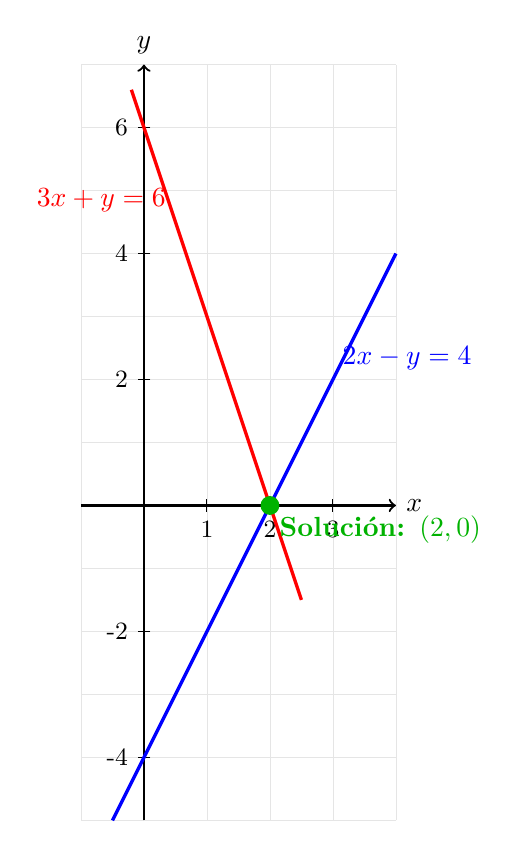
\begin{tikzpicture}[scale=0.8]
    % Grid
    \draw[gray!20, very thin] (-1,-5) grid (4,7);

    % Axes
    \draw[->, thick] (-1,0) -- (4,0) node[right] {$x$};
    \draw[->, thick] (0,-5) -- (0,7) node[above] {$y$};

    % Axis labels
    \foreach \x in {1,2,3}
        \draw (\x,0.1) -- (\x,-0.1) node[below, font=\small] {\x};
    \foreach \y in {-4,-2,2,4,6}
        \draw (0.1,\y) -- (-0.1,\y) node[left, font=\small] {\y};

    % First line: 2x - y = 4  (or y = 2x - 4)
    \draw[blue, very thick, domain=-0.5:4] plot (\x, {2*\x - 4});
    \node[blue, above right] at (3,2) {$2x - y = 4$};

    % Second line: 3x + y = 6  (or y = -3x + 6)
    \draw[red, very thick, domain=-0.2:2.5] plot (\x, {-3*\x + 6});
    \node[red, above left] at (0.5,4.5) {$3x + y = 6$};

    % Intersection point
    \filldraw[green!70!black] (2,0) circle (4pt);
    \node[green!70!black, below right] at (2,0) {\textbf{Solución: $(2, 0)$}};
\end{tikzpicture}
\end{center}

\textbf{Solución:} El punto de intersección es $(2, 0)$.

\textbf{Verificación:}
\begin{itemize}
    \item $2(2) - 0 = 4 - 0 = 4$ \quad $\checkmark$
    \item $3(2) + 0 = 6 + 0 = 6$ \quad $\checkmark$
\end{itemize}
\end{example}

\newpage
%========================================
% SECTION 12.3: Método de Sustitución
%========================================
\subsectiontitle{Método de Sustitución}

El método de sustitución es un proceso algebraico que permite resolver sistemas de ecuaciones sin necesidad de graficar.

\begin{theorem}
\textbf{Método de Sustitución:}

\begin{enumerate}
    \item \textbf{Despejar una incógnita:} Escoja una ecuación y despeje una incógnita en términos de la otra incógnita.

    \item \textbf{Sustituir:} Sustituya la expresión hallada en el paso anterior en la otra ecuación para obtener una ecuación con una sola incógnita y, a continuación, despeje esa incógnita.

    \item \textbf{Sustituir a la inversa:} En la expresión hallada en el primer paso, sustituya el valor hallado para despejar la incógnita restante.

    \item \textbf{Verificar:} Compruebe la solución sustituyendo los valores en ambas ecuaciones originales.
\end{enumerate}
\end{theorem}

\begin{example}
\textbf{Resolver por sustitución el sistema}

$$\begin{cases}
2x - y = 4 \\
3x + y = 6
\end{cases}$$

\textbf{Paso 1: Despejar una incógnita}

Despejamos $y$ de la primera ecuación:
\begin{align*}
2x - y &= 4 \\
-y &= 4 - 2x \\
y &= 2x - 4
\end{align*}

\textbf{Paso 2: Sustituir}

Sustituimos $y = 2x - 4$ en la segunda ecuación:
\begin{align*}
3x + y &= 6 \\
3x + (2x - 4) &= 6 \\
5x - 4 &= 6 \\
5x &= 10 \\
x &= 2
\end{align*}

\textbf{Paso 3: Sustituir a la inversa}

Sustituimos $x = 2$ en la expresión $y = 2x - 4$:
\begin{align*}
y &= 2(2) - 4 \\
y &= 4 - 4 \\
y &= 0
\end{align*}

\textbf{Paso 4: Verificar}

Verificamos la solución $(2, 0)$ en ambas ecuaciones:
\begin{itemize}
    \item Primera ecuación: $2(2) - 0 = 4$ \quad $\checkmark$
    \item Segunda ecuación: $3(2) + 0 = 6$ \quad $\checkmark$
\end{itemize}

\textbf{Solución del sistema:} $(x, y) = (2, 0)$
\end{example}

\newpage
%========================================
% SECTION 12.4: Método de Eliminación
%========================================
\subsectiontitle{Método de Eliminación (o Método de Suma y Resta)}

El método de eliminación consiste en sumar o restar las ecuaciones para eliminar una de las variables.

\begin{theorem}
\textbf{Método de Eliminación:}

\begin{enumerate}
    \item \textbf{Ajustar los coeficientes:} Multiplique una o más de las ecuaciones por números apropiados, de modo que el coeficiente de una incógnita de una ecuación sea el \textbf{opuesto} (negativo) de su coeficiente en la otra ecuación.

    \item \textbf{Sumar las ecuaciones:} Sume las dos ecuaciones para eliminar una incógnita y, a continuación, despeje la incógnita restante.

    \item \textbf{Sustituir a la inversa:} En una de las ecuaciones originales, sustituya el valor hallado y despeje la incógnita restante.

    \item \textbf{Verificar:} Compruebe la solución sustituyendo los valores en ambas ecuaciones originales.
\end{enumerate}
\end{theorem}

\begin{example}
\textbf{Resolver por eliminación el sistema}

$$\begin{cases}
2x - y = 4 \\
3x + y = 6
\end{cases}$$

\textbf{Paso 1: Ajustar los coeficientes}

Observamos que los coeficientes de $y$ son $-1$ y $+1$, que ya son opuestos. No necesitamos multiplicar por ningún número.

\textbf{Paso 2: Sumar las ecuaciones}

Sumamos ambas ecuaciones:
\begin{align*}
(2x - y) + (3x + y) &= 4 + 6 \\
2x - y + 3x + y &= 10 \\
5x + 0y &= 10 \\
5x &= 10 \\
x &= 2
\end{align*}

\textbf{Paso 3: Sustituir a la inversa}

Sustituimos $x = 2$ en la primera ecuación original:
\begin{align*}
2(2) - y &= 4 \\
4 - y &= 4 \\
-y &= 0 \\
y &= 0
\end{align*}

\textbf{Paso 4: Verificar}

Verificamos la solución $(2, 0)$ en ambas ecuaciones:
\begin{itemize}
    \item Primera ecuación: $2(2) - 0 = 4$ \quad $\checkmark$
    \item Segunda ecuación: $3(2) + 0 = 6$ \quad $\checkmark$
\end{itemize}

\textbf{Solución del sistema:} $(x, y) = (2, 0)$
\end{example}

\newpage

\begin{example}
\textbf{Resolver por eliminación cuando se requiere ajustar coeficientes}

$$\begin{cases}
3x + 2y = 8 \\
5x - 3y = 1
\end{cases}$$

\textbf{Paso 1: Ajustar los coeficientes}

Decidimos eliminar $y$. Los coeficientes de $y$ son 2 y $-3$.

Multiplicamos la primera ecuación por 3 y la segunda por 2:

\textbf{Primera ecuación} $\times 3$:
$$3(3x + 2y) = 3(8) \implies 9x + 6y = 24$$

\textbf{Segunda ecuación} $\times 2$:
$$2(5x - 3y) = 2(1) \implies 10x - 6y = 2$$

Ahora los coeficientes de $y$ son $+6$ y $-6$ (opuestos).

\textbf{Paso 2: Sumar las ecuaciones}

\begin{align*}
(9x + 6y) + (10x - 6y) &= 24 + 2 \\
19x + 0y &= 26 \\
19x &= 26 \\
x &= \frac{26}{19}
\end{align*}

\textbf{Paso 3: Sustituir a la inversa}

Sustituimos $x = \frac{26}{19}$ en la primera ecuación original:
\begin{align*}
3\left(\frac{26}{19}\right) + 2y &= 8 \\
\frac{78}{19} + 2y &= 8 \\
2y &= 8 - \frac{78}{19} \\
2y &= \frac{152 - 78}{19} \\
2y &= \frac{74}{19} \\
y &= \frac{37}{19}
\end{align*}

\textbf{Solución del sistema:} $(x, y) = \left(\dfrac{26}{19}, \dfrac{37}{19}\right)$
\end{example}

\newpage
%========================================
% SECTION 12.5: Número de Soluciones
%========================================
\subsectiontitle{Número de Soluciones de un Sistema Lineal}

\begin{theorem}
\textbf{Clasificación de Sistemas de Ecuaciones Lineales:}

Para un sistema de dos ecuaciones lineales con dos incógnitas, \textbf{exactamente una} de las siguientes afirmaciones es verdadera:

\begin{enumerate}
    \item \textbf{El sistema tiene exactamente una solución} (las rectas se intersectan en un punto).
    \item \textbf{El sistema no tiene solución} (las rectas son paralelas).
    \item \textbf{El sistema tiene un número infinito de soluciones} (las rectas coinciden).
\end{enumerate}
\end{theorem}

\textbf{Representación Gráfica de los Tres Casos:}

\begin{center}
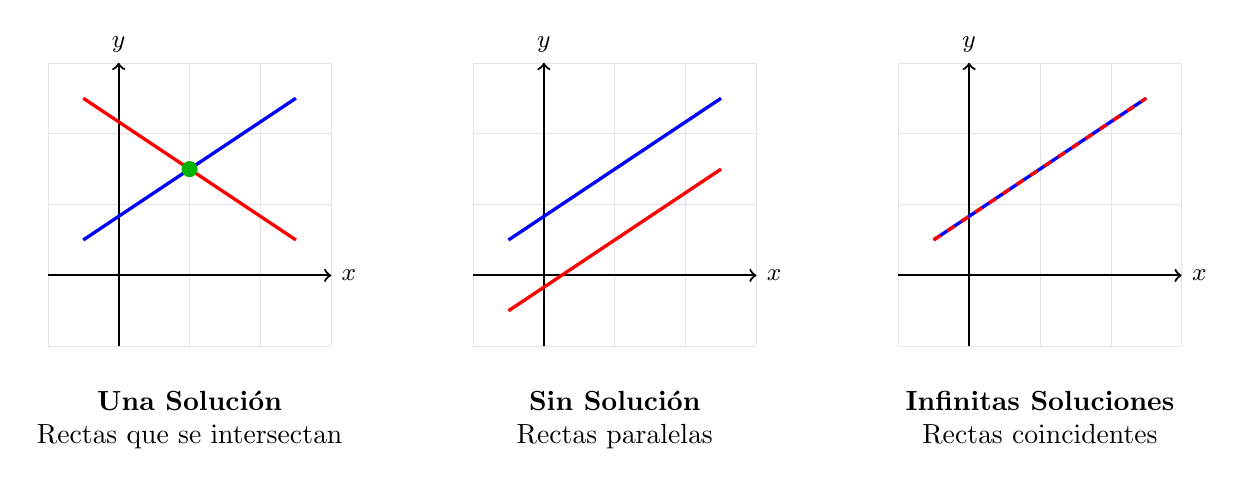
\begin{tikzpicture}[scale=0.9]
    % Case 1: One solution (intersecting lines)
    \begin{scope}[xshift=0cm]
        \draw[gray!20, very thin] (-1,-1) grid (3,3);
        \draw[->, thick] (-1,0) -- (3,0) node[right, font=\small] {$x$};
        \draw[->, thick] (0,-1) -- (0,3) node[above, font=\small] {$y$};

        \draw[blue, very thick] (-0.5,0.5) -- (2.5,2.5);
        \draw[red, very thick] (-0.5,2.5) -- (2.5,0.5);

        \filldraw[green!70!black] (1,1.5) circle (3pt);

        \node[below, align=center] at (1,-1.5) {\textbf{Una Solución} \\ Rectas que se intersectan};
    \end{scope}

    % Case 2: No solution (parallel lines)
    \begin{scope}[xshift=6cm]
        \draw[gray!20, very thin] (-1,-1) grid (3,3);
        \draw[->, thick] (-1,0) -- (3,0) node[right, font=\small] {$x$};
        \draw[->, thick] (0,-1) -- (0,3) node[above, font=\small] {$y$};

        \draw[blue, very thick] (-0.5,0.5) -- (2.5,2.5);
        \draw[red, very thick] (-0.5,-0.5) -- (2.5,1.5);

        \node[below, align=center] at (1,-1.5) {\textbf{Sin Solución} \\ Rectas paralelas};
    \end{scope}

    % Case 3: Infinite solutions (coincident lines)
    \begin{scope}[xshift=12cm]
        \draw[gray!20, very thin] (-1,-1) grid (3,3);
        \draw[->, thick] (-1,0) -- (3,0) node[right, font=\small] {$x$};
        \draw[->, thick] (0,-1) -- (0,3) node[above, font=\small] {$y$};

        \draw[blue, very thick] (-0.5,0.5) -- (2.5,2.5);
        \draw[red, very thick, dashed] (-0.5,0.5) -- (2.5,2.5);

        \node[below, align=center] at (1,-1.5) {\textbf{Infinitas Soluciones} \\ Rectas coincidentes};
    \end{scope}
\end{tikzpicture}
\end{center}

\begin{example}
\textbf{Identificar el número de soluciones}

\textbf{a) Sistema con una solución:}
$$\begin{cases}
x + y = 5 \\
x - y = 1
\end{cases}$$

Las rectas tienen diferentes pendientes y se intersectan en un punto. \textbf{Una solución:} $(3, 2)$.

\textbf{b) Sistema sin solución:}
$$\begin{cases}
2x + y = 4 \\
2x + y = 7
\end{cases}$$

Ambas ecuaciones tienen la misma forma ($2x + y =$) pero diferentes constantes (4 y 7). Las rectas son paralelas. \textbf{Sin solución.}

\textbf{c) Sistema con infinitas soluciones:}
$$\begin{cases}
2x + 4y = 8 \\
x + 2y = 4
\end{cases}$$

Si multiplicamos la segunda ecuación por 2, obtenemos la primera ecuación. Las rectas coinciden. \textbf{Infinitas soluciones.}
\end{example}

\newpage
%========================================
% SECTION 12.6: Modelado con Sistemas Lineales
%========================================
\subsectiontitle{Modelado con Sistemas Lineales}

Los sistemas de ecuaciones lineales son herramientas poderosas para resolver problemas del mundo real.

\begin{theorem}
\textbf{Proceso para Resolver Problemas con Sistemas de Ecuaciones:}

\begin{enumerate}
    \item \textbf{Identificar las variables:} Identifique las cantidades que el problema pide hallar. Introduzca notación para las variables (por ejemplo, $x$ e $y$).

    \item \textbf{Expresar todas las cantidades desconocidas en términos de las variables:} Exprese todas las cantidades mencionadas en el problema en términos de las variables definidas.

    \item \textbf{Establecer un sistema de ecuaciones:} Encuentre los datos cruciales del problema que den las relaciones entre las expresiones y establezca un sistema de ecuaciones (un modelo) que exprese estas relaciones.

    \item \textbf{Resolver el sistema e interpretar los resultados:} Resuelva el sistema usando cualquiera de los métodos aprendidos, verifique sus soluciones y dé su respuesta final como una frase que conteste la pregunta planteada en el problema.
\end{enumerate}
\end{theorem}

\begin{example}
\textbf{Problema de suma y diferencia}

Encuentre dos números cuya suma es 34 y cuya diferencia es 10.

\textbf{Paso 1: Identificar las variables}

Sea $x$ el número mayor y $y$ el número menor.

\textbf{Paso 2: Expresar las cantidades}

\begin{itemize}
    \item La suma de los números es 34: $x + y = 34$
    \item La diferencia de los números es 10: $x - y = 10$
\end{itemize}

\textbf{Paso 3: Establecer el sistema}

$$\begin{cases}
x + y = 34 \\
x - y = 10
\end{cases}$$

\textbf{Paso 4: Resolver el sistema}

Usando el método de eliminación (sumamos las ecuaciones):
\begin{align*}
(x + y) + (x - y) &= 34 + 10 \\
2x &= 44 \\
x &= 22
\end{align*}

Sustituimos en la primera ecuación:
\begin{align*}
22 + y &= 34 \\
y &= 12
\end{align*}

\textbf{Verificación:}
\begin{itemize}
    \item Suma: $22 + 12 = 34$ \quad $\checkmark$
    \item Diferencia: $22 - 12 = 10$ \quad $\checkmark$
\end{itemize}

\textbf{Respuesta:} Los dos números son 22 y 12.
\end{example}

\begin{example}
\textbf{Problema de monedas}

Un hombre tiene 14 monedas en su bolsillo, todas las cuales son de 10 o de 25 centavos. Si el valor total de su cambio es \$2.75, ¿cuántas monedas de 10 centavos y cuántas de 25 centavos tiene?

\textbf{Paso 1: Identificar las variables}

Sea:
\begin{itemize}
    \item $x$ = número de monedas de 10 centavos
    \item $y$ = número de monedas de 25 centavos
\end{itemize}

\textbf{Paso 2: Expresar las cantidades}

\begin{itemize}
    \item Total de monedas: $x + y = 14$
    \item Valor total (en centavos): $10x + 25y = 275$
\end{itemize}

\textbf{Paso 3: Establecer el sistema}

$$\begin{cases}
x + y = 14 \\
10x + 25y = 275
\end{cases}$$

\textbf{Paso 4: Resolver el sistema}

Despejamos $x$ de la primera ecuación:
$$x = 14 - y$$

Sustituimos en la segunda ecuación:
\begin{align*}
10(14 - y) + 25y &= 275 \\
140 - 10y + 25y &= 275 \\
140 + 15y &= 275 \\
15y &= 135 \\
y &= 9
\end{align*}

Sustituimos para hallar $x$:
$$x = 14 - 9 = 5$$

\textbf{Verificación:}
\begin{itemize}
    \item Total de monedas: $5 + 9 = 14$ \quad $\checkmark$
    \item Valor total: $10(5) + 25(9) = 50 + 225 = 275$ centavos = \$2.75 \quad $\checkmark$
\end{itemize}

\textbf{Respuesta:} El hombre tiene 5 monedas de 10 centavos y 9 monedas de 25 centavos.
\end{example}
